% !TEX root = main.tex

\begin{itemize}
\item The analysis is performed according to ISO 14040, ISO 14044 and ISO 15804. % 15804 to be discussed
	\item The impact category, which will be evaluated, is the global warming potential (GWP). This is described as the emissions of ${\mathrm{CO_2-eq}}$ in kilograms divided by the functional unit.
	\item The functional unit used is twofold and based on the function of the adaptive building envelope. For the comparison with other shading systems facade area in ${\mathrm{m^2}}$ is used, while comparison with other photovoltaic systems is done using electricity produced in ${\mathrm{kWh}}$. According to the guidelines of the International Energy Agency (IEA), the calculation of kWh produced needs to be based for consistency on conversion efficiency ${\eta}$, performance ratio PR, irradiation I, lifetime LT and area A of the module. Equation \ref{eq:solar} gives the exact formulation:
	% Variables in italics?
	% LT - service life?
\begin{equation}
G=\frac{{\mathrm{GWP}}}{{\mathrm{I \cdot \eta  \cdot PR \cdot LT \cdot A}}}
% what is G
\label{eq:solar}
\end{equation}

	\item The LCI inventory was obtained through...

	\item The scope of the LCA comprises the embodied, operational and disposal global warming impact of the respective system. Figure \ref{fig:BOS} illustrates the system boundaries of the process flows. The supporting structures are also included in the system boundaries. The reason for this is that technologies within the building envelope also change the design of the supporting structures. The supporting structure of solar panels is referred to as balance of systems (BOS).
% We will need to describe a little more what is included and what is not, i.e.
%   not only supporting structure

\begin{figure}[H]
\begin{center}
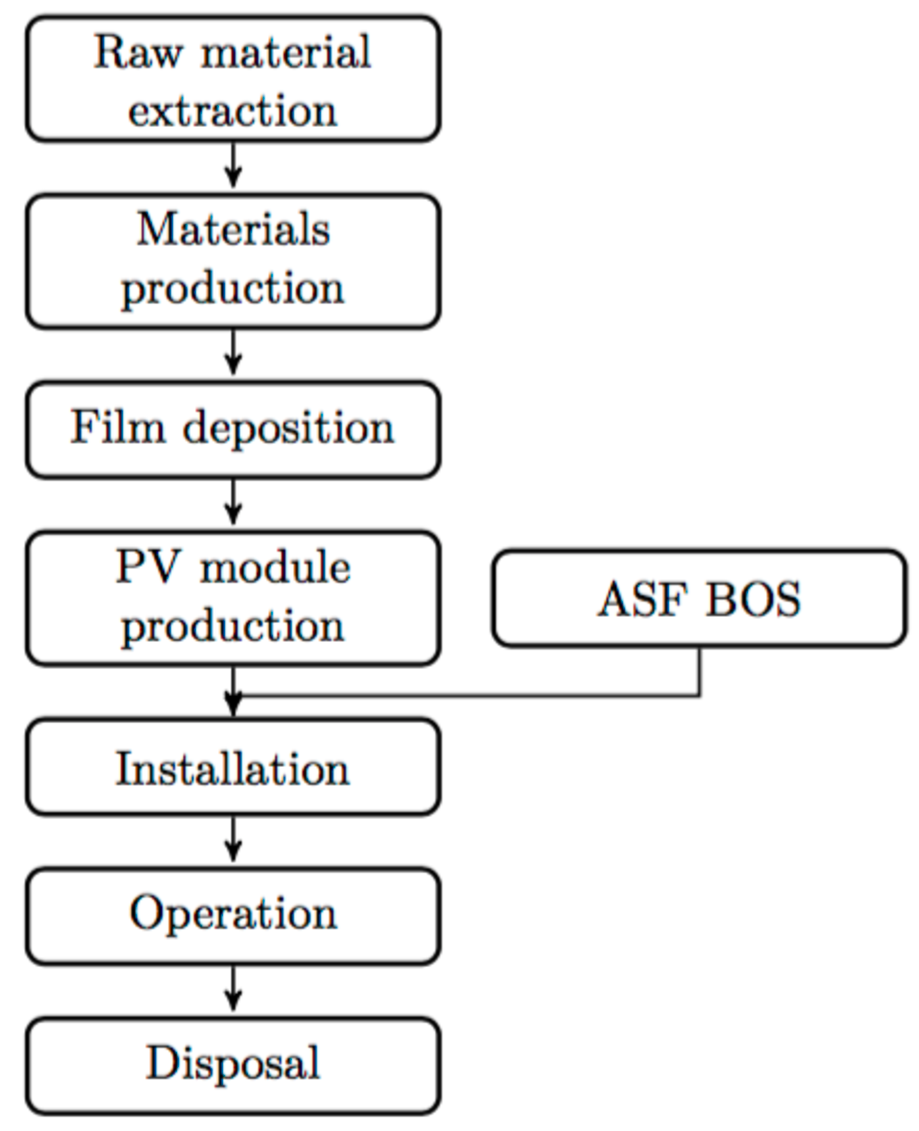
\includegraphics[width=5cm, trim= 0cm 0cm 0cm 0cm,clip]{BOS}
\caption{Thin-film incl. BOS system boundaries}
\label{fig:BOS}
\end{center}
\end{figure}

	\item The cut-off approach is used for recycling and landfill. This means that recycling does not generate any credit for the product and resulting benefits are not taken into account. Furthermore the use of recycled products do not bear the burden of processes higher up the chain.
	% we may need to discuss system expansion
	% PV electricity production not included?
	\item The recipe midpoint (H) allocation method allows for an accurate evaluation of the GWP based on human impact factors.
	% I don't get it - sorry
	% I am pretty sure ReciPe basically uses the IPCC method
\item The adaptive solar facade uses CIGS thin film panels with an aluminum backing. This allows for a light-weight panel, needed for the flexible control of the system using silicone soft-robotic actuators.
% move this point up the list
\end{itemize}

\begin{figure}[H]
\begin{center}
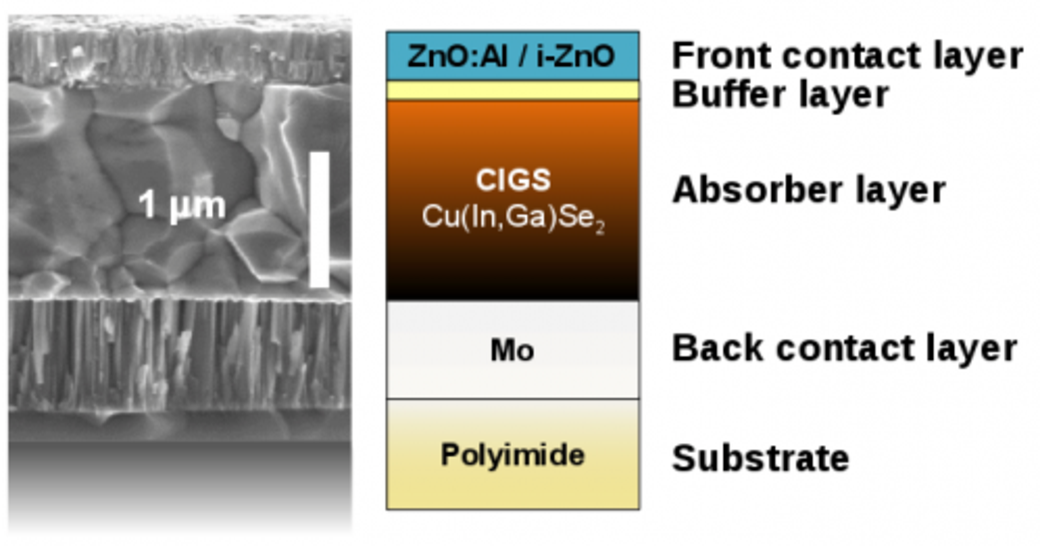
\includegraphics[width=8cm, trim= 0cm 0cm 0cm 0cm,clip]{schema}
\caption{CIGS thin film structure}
\label{fig:schema}
\end{center}
\end{figure}

% what LCI DB (ecoinvent) is used? refer to Annex?
% How was LCI data collected?
% see above. Explain what is included and excluded
